\documentclass{article}[18pt]
\usepackage{../../../format}
\lhead{A Level Physics - Fields}

%File specific Preamble
\usetikzlibrary{decorations, decorations.text}

\begin{document}
\begin{center}
\underline{\huge Magnetic Fields}
\end{center}
\section{Charged Particles in magnetic fields}
Force is always perpendicular to the direction - no change in speed to the electrons.\\
\\
If electrons are confined to a wire $F=BIl$\\
\\
The same equation applies for many charges where:
$$I=\frac{Q}{t} \quad l=vt$$
$$F=B\times\frac{Q}{t}\times vt$$
$$F=BQv$$
\subsection{The hall probe}
This is used to measure the strength of magnetic fields. It consists of a thin slice of semiconductor material with a constant current flowing through it.\\
\\
The negative charges go to the bottom of the material and so the top is positively charged, this creates a potential difference.
$$F_B=F_E$$
$$BQV=\frac{VQ}{d}$$
$$V=Bvd$$
$$V\propto B$$
By measuring the voltage across the probe the magnetic field strength can be measured.
\section{Charged particles in circular orbits}
\textbf{Force} will always be perpendicular to the direction of motion\\
No work is done by the magnetic field on the particles\\
\\
Direction changes but not speed\\
Constant kinetic energy\\
\\
Path is circular\\
Causes a centripetal acceleration\\
$$F=BQv=\dfrac{mv^2}{r}$$
$$r=\dfrac{mv}{BQ}$$
\newpage
\section{Applications}
\subsection{Cyclotron}
This is used in hospitals to produce high energy beams for radiotherapy.\\
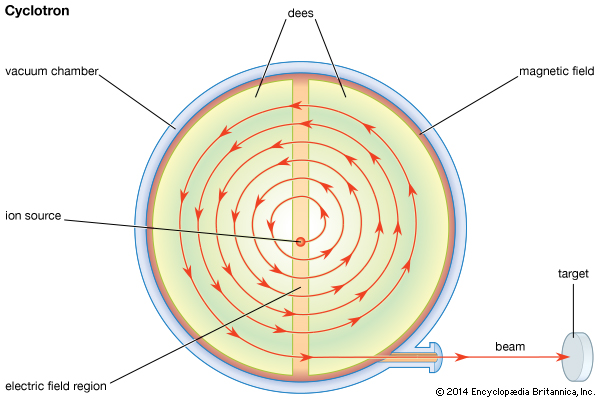
\includegraphics[width=10cm]{cyclotron.jpg}\\
\begin{itemize}
\item Proton source in centre
\item Electric field in between C Cores to accelerate protons
\item Magnetic field causes curved path
\item r increases as v increases
\end{itemize}
\subsection{Mass Spectrometer}
This is used to analyse the type of atoms present in a sample\\
\\
\\
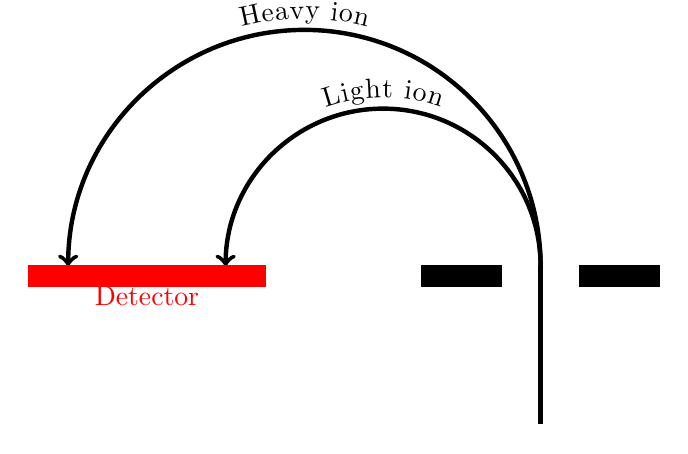
\begin{tikzpicture}
\draw[ultra thick, ->,postaction={decorate, decoration={text along path, raise=4pt, text align={align=center}, text={Light ion}, reverse path}}] (6.5,0) arc (0:180:2);
\draw[ultra thick, ->,postaction={decorate, decoration={text along path, raise=4pt, text align={align=center}, text={Heavy ion}, reverse path}}] (6.5,0) arc (0:180:3);
\draw[red,thick,fill=red] (0,0)rectangle (3,-0.25) node[below,midway] {Detector};
\draw[black,fill=black,thick] (5,0)rectangle (6,-0.25);
\draw[black,fill=black,thick] (7,0)rectangle (8,-0.25);
\draw[black,ultra thick] (6.5,0) -- (6.5,-2);
\end{tikzpicture}
\\
\begin{itemize}
\item Magnetic field out of diagram
\item Atoms in the sample are ionised
\item Directed in a narrow beam into the magnetic field
\item Radius of path depends on specific charge
\end{itemize}
$$r=\dfrac{mv}{BQ}$$
$$r\propto\dfrac{1}{\frac{q}{m}}$$
\subsubsection{Velocity selector}
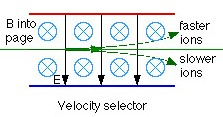
\includegraphics[width=10cm]{velocity_selector.jpg}\\
Negative ions fall to the bottom surface, causing the top surface to have a positive charge, creating a potential difference. For an ion to continue on a straight path the force from the magnetic field up must be equal to the force from the electric field down.\\
$$F=BQv=EQ$$
$$BQv=\dfrac{V}{d}Q$$
$$v=\dfrac{V}{Bd}$$
This means that only particles of speed $v$ will travel through the gap

\end{document}